\documentclass[10pt,a4paper]{report}
\usepackage[latin1]{inputenc}
\usepackage{amsmath}
\usepackage[margin=20mm]{geometry}
\usepackage{amsfonts}
\usepackage{amssymb}
\usepackage{graphicx}
\usepackage{float}
\begin{document}
	\begin{titlepage}
		\begin{minipage}{0.5\textwidth}
			\begin{figure}[H]
				\includegraphics[scale=0.20]{../UofK.JPG}\\
				[2cm]
			\end{figure}
		\end{minipage} \hfill
		\begin{minipage}{0.45\textwidth}
			\textsc{\LARGE University of Khartoum }\\
				[2mm]
				\textsc{\LARGE Faculty of Science } \\
				[1mm]
				\textsc{\Large Physics Department } \\
				[2mm]
				{\large Physics Lab - Year 3} \\ 
				[3mm]
		\end{minipage} 

		\begin{center}
			{\large Lab Report: } \\
			\line(1,0){350} \\
			[0.15in]
			\textbf{{\huge Specific charge of the electron $e/m$ }} \\
			[0.10in]
			\line(1,0){260} \\ [10cm]
		\end{center}
		
		\begin{flushleft}
				Written By:  \\
				{\large
							 Tariq Mohamed Hashim Erwa \\
							 Group B \\}
							 March, 9, 2021
		\end{flushleft}
	\end{titlepage}

\section*{\textbf{{Objective:}}}
   {\large To determine the specific of an 
   electron {\Large $e/m$}}

\section*{\textbf{{Apparatus:}}} 
   {\large $e/m$ apparatus, Power 
   supplies for the apparatus, Voltmeter and ammeter.}

\section*{\textbf{{Theory:}}} 
	{\large A hot filament is used as the electrons source.
	 The emitted electrons are accelerated using an anode.\\
		The kinetic energy gained by the electrons is:
		\begin{equation}
			eU=\frac{1}{2}mv^{2}\\
		\end{equation}\
		Where e and m are the charge and mass of the electron respectively,\\
		$U \equiv$ accelerating potential.\\
		$v \equiv$ electron velocity.\\
		The accelerated electrons are now subjected to external magnetic field
		 perpendicular to the direction of the electrons, as shown in the figure below}   
		\begin{figure}[h]
			\centering
			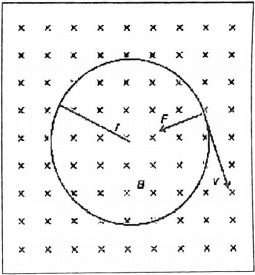
\includegraphics[width=5cm]{e-m}
			\caption[ljglk]{accelerated electron path in magnetic field}
		\end{figure}
		
	
	{\large The force acting on the electron is given by Lorentz force
	$$\vec{F}=e\vec{v}\times \vec{B}$$
	where $\vec{B}$ is the external magnetic field. Since $\vec{v}$ 
	and $\vec{B}$ are perpendicular we get
	$$\vec{F}=evB.$$\
	The force will be centripetal, i.e. it will be directed towards the center,
	 The electron trajectory is circular. We can now write
		\begin{equation}
			m \frac{v^{2}}{r}=evB
		\end{equation}
	where $r$ is the radius of the circular orbit.\\
	The electron velocity can't be found in this experiment, so we use equations 
	(1) and (2) to eliminate it and we get:
		\begin{equation}
			r^{2}=\frac{2U}{(e/m)B^{2}}
		\end{equation}
	The source of the external magnetic field is a pair of Helmholtz coils. 
	The magnetic field in the coils is produced when a current is passed through
	 the coils. The magnetic field strength can be written as
		\begin{equation*}
	B=kI,
		\end{equation*}
	where $k$ is a constant depending on the geometry and setup of the coils used, 
	$I\equiv the current passing through the coils.$\\
	For the Helmholtz coils $k$ is given by
		\begin{equation*}
	k=\mu_{\circ}(\frac{4}{5})^{\frac{3}{2}}.n.R
		\end{equation*}
	where $\mu_{\circ}=4\pi \times 10^{-7}V.s/A$m:(magnetic field constant),\\
	$n\equiv$ number of turns in each coil: ($ n $= 130 turn/coil)\\ 
	$R\equiv$ Radius of coils: ($R$= 150mm).\\
	Now (3) can be written as:
		\begin{equation}
	r^{2}=\frac{2U}{(e/m)k^{2}I^{2}} 
		\end{equation}
	We notice that the radius of the circular orbit is depending on the applied
	 potential and current.\\
	The tube is filled with hydrogen molecules at low pressure, which through 
	collision with electrons are caused to emit light.}

\section*{\textbf{{Results:}}}
	{\Large 
		\begin{center}
			\begin{tabular}{|c|c|c||c|c|}
				\hline%caption?
				$I_{(A)}$ & $I^{2}_{(A^{2})}$ & $\frac{1}{I^{2}}_{(A^{-2})}$ & $r_{(cm)}$ & $r^{2}_{(cm^{2})}$ \\
				\hline
				1.0 & 1.0 & 1.0 & 3.05 & 9.30 \\
				\hline
				1.1 & 1.21 & 0.83 & 2.85 & 8.12 \\
				\hline
				1.2 & 1.44 & 0.69 & 2.65 & 7.02 \\
				\hline
				1.3 & 1.69 & 0.59 & 2.5 & 6.25 \\
				\hline
				1.4 & 1.96 & 0.51 & 2.3 & 5.29 \\
				\hline
				1.5 & 2.25 & 0.44 & 2.25 & 5.06 \\
				\hline
				1.6 & 2.56 & 0.39 & 1.85 & 3.42 \\
				\hline
			\end{tabular}\\
			Table 1 : shows the readings from $e/m$ apparatus and ammeter \\
		\end{center}}
	
\section*{\textbf{{Calculations:}}}
	\begin{center}
		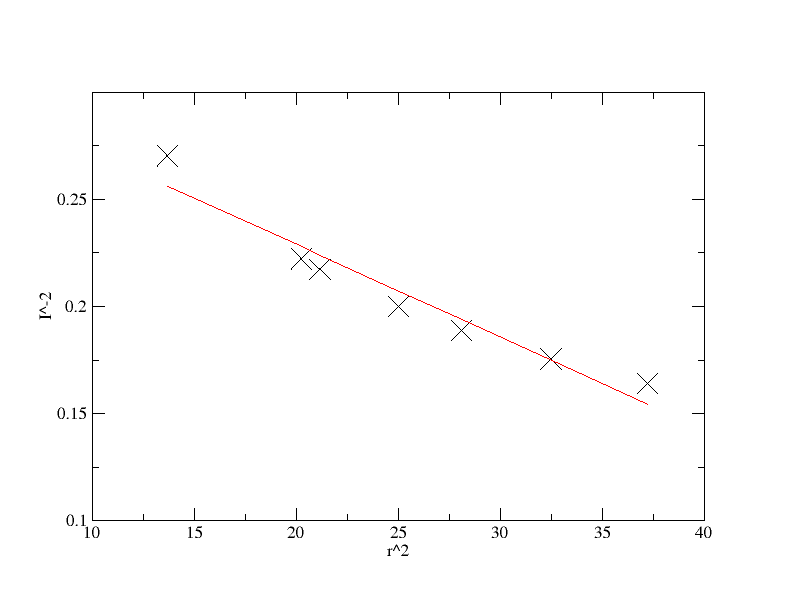
\includegraphics[scale = 0.4]{graph.png}\\
		Figure 1 : shows the plot of $r^2$ vs $\frac{1}{I^2}$
	\end{center}
	{\large looking at (4) we notice that we can vary $U$ , While keeping $I$ 
	constant or the other way around to vary $I$ , While keeping $U$ constant.
	 We use the second method in this experiment, by rearranging equation (4) 
	 we get:
	$$\frac{r^{2}}{I^{2}}=\frac{2U}{(e/m)k^{2}}$$ 
	from Figure 1 we get a straight line with slope
	\begin{align*}
		T & = \frac{2U}{(e/m)k^{2}}\\
		& = -0.0043353
	\end{align*}

	where $$k=0.0175334204$$ 
	%should add T & k here
	$$\therefore e/m=\frac{2\times 300}{-0.0043353\times 0.0175334204} Colomb/kg$$
	
\pagebreak
\section*{\textbf{{Method:}}}
   After connecting the circuit of The $e/m$ apparatus ,
   the Ammeter and the Voltmeter. The voltage was set constant to 300V
   and the current was tuned to known values, for each value the radius 
   of the Cathode circule was read from the $e/m$ apparatus rule.

\section*{\textbf{{Conclusion:}}}
{\large The specific of an electron was determined to be }
$ = \underline{\underline{-0.451109716 \times 10 ^9$} Colomb/kg

\end{document}
